% -*-coding: utf-8 -*-
% Держать в начале каждого файла!

\documentclass[a4paper, 12pt]{extarticle}
\usepackage{metod}

\MTDSetPhysSection{Механика}
\MTDSetTitle{Определение коэффициента трения качения}
\MTDDesignator{М--8}
\MTDSetGrade{10}

\MTDSetAuthors{И.~Н.~Грачева, В.~И.~Гребенкин, А.~Е.~Иванов, И.~А.~Коротова,
Е.~И.~Красавина, А.~В.~Кравцов, Н.~С.~Кулеба, Б.~В.~Падалкин,
Г.~Ю.~Шевцова, Т.~С.~Цвецинская}

\MTDSetEditorsGenCase{И.~Н.~Грачевой, А.~Е.~Иванова, А.~В.~Кравцова}

%\newcommand{\eps}{\epsilon}

\begin{document}

\MTDTitlePage
\MTDInfoPage

\setcounter{section}{8}

\subsection{Цель работы}
Целью работы является экспериментальное определение коэффициента трения качения шара по плоской пластине при различных углах наклона пластины.

\subsection{Основные теоретические сведения}
При качении по плоской поверхности тел, имеющих форму круговых цилиндров или шаров, возникают не только упругие, но и пластические деформации. Из-за этого линия действия реакции опорной поверхности не совпадает с линией действия нормального давления. Направление линии  действия реакции опорной поверхности качественно может быть определено из следующих соображений.

\begin{figure}[h]
\begin{center}
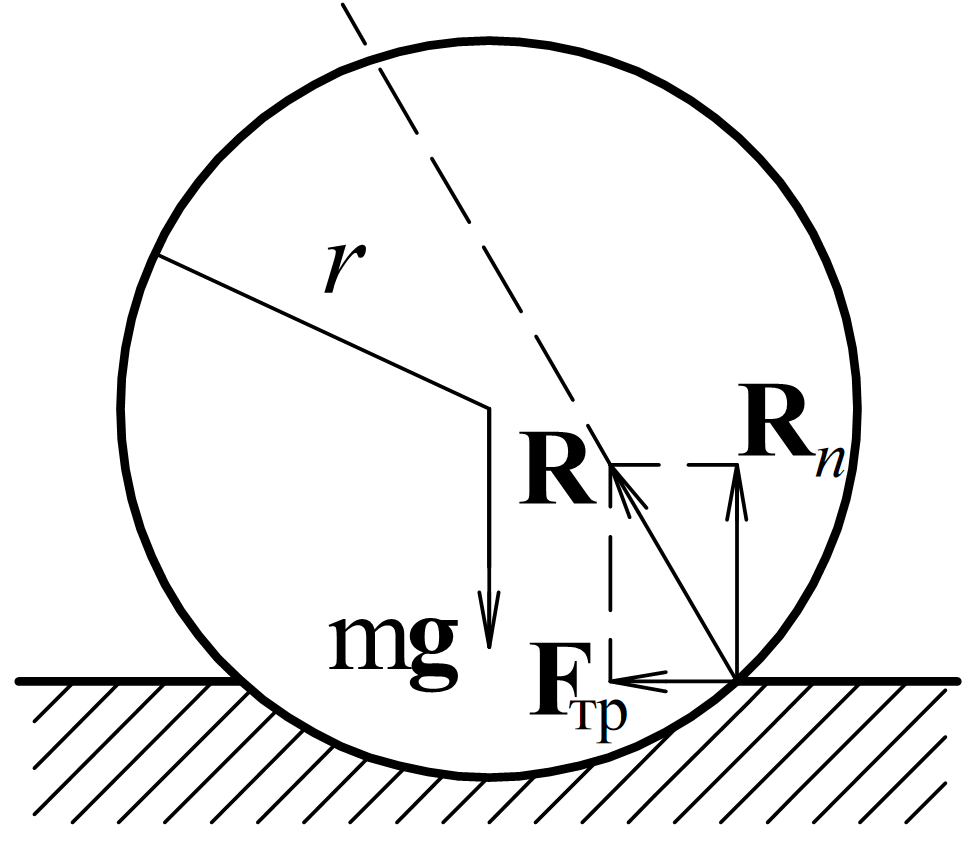
\includegraphics[scale = 0.21, keepaspectratio=true]{M8-RollingMotionForces}
\end{center}
\caption{Силы, действующие при качении \label{fig:m8-rolling}}
\end{figure}

\begin{figure}[h]
\begin{center}
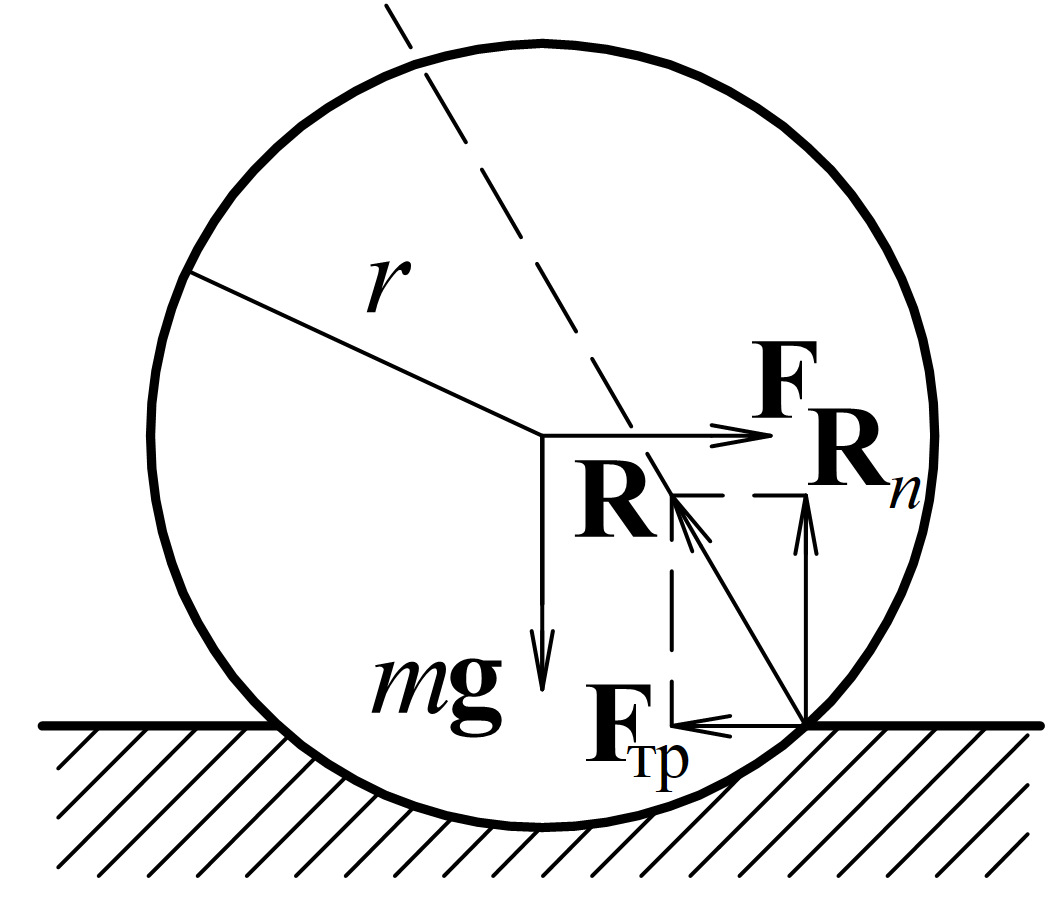
\includegraphics[scale = 0.21, keepaspectratio=true]{M8-SteadyRollingMotionForces}
\end{center}
\caption{Силы, действующие при равномерном качении \label{fig:m8-uniform-rolling}}
\end{figure}
% Надо рядышком их

Сила трения является диссипативной силой, следовательно, центр масс тела движется замедленно, а угловое ускорение направлено противоположно угловой скорости. Для соблюдения этих условий точка приложения реакции опорной  поверхности должна находиться впереди (относительно перемещения) центра масс, а сама сила реакции опоры должна быть направлена вверх-назад причем линия действия этой силы должна проходить впереди центра масс (рис.~\ref{fig:m8-rolling}). В случае равномерного качения под действием силы~$F$ (рис.~\ref{fig:m8-uniform-rolling}) нормальная к плоскости составляющая $R_n$ реакции опорной поверхности~$R$ численно равна $mg$, где $m$ "--- масса тела, а горизонтальная составляющая~$F_\text{тр}$ является силой трения качения, равную (по Кулону) %равнУЮ?! | РавнОЙ :)
\begin{equation}
\label{eq:m8-rolling-resistance}
F_\text{тр} = f_\text{к} \frac{R_n}{r}, %k или к? везде по-разному. это значит "коэффициент"?
\end{equation}
где $f_\text{к}$ "--- коэффициент трения качения, имеющий размерность длины и зависящий при качении от материалов тел, состояния их поверхностей и ряда других факторов;
$r$ - радиус катящегося тела.

Пара сил $R_n$ и $F_n$, приложенных к катящемуся телу, создает момент трения
\begin{equation}
\label{eq:m8-friction-moment}
M_\text{тр} = F_\text{тр}r = f_\text{к} R_n,
\end{equation}
Из выражения~\eqref{eq:m8-friction-moment} видно, что $f_\text{к}$ численно равен плечу $R_n$, т.~e. расстоянию от линии действия $R_n$ до оси вращения.

\begin{figure}[h]
\begin{center}
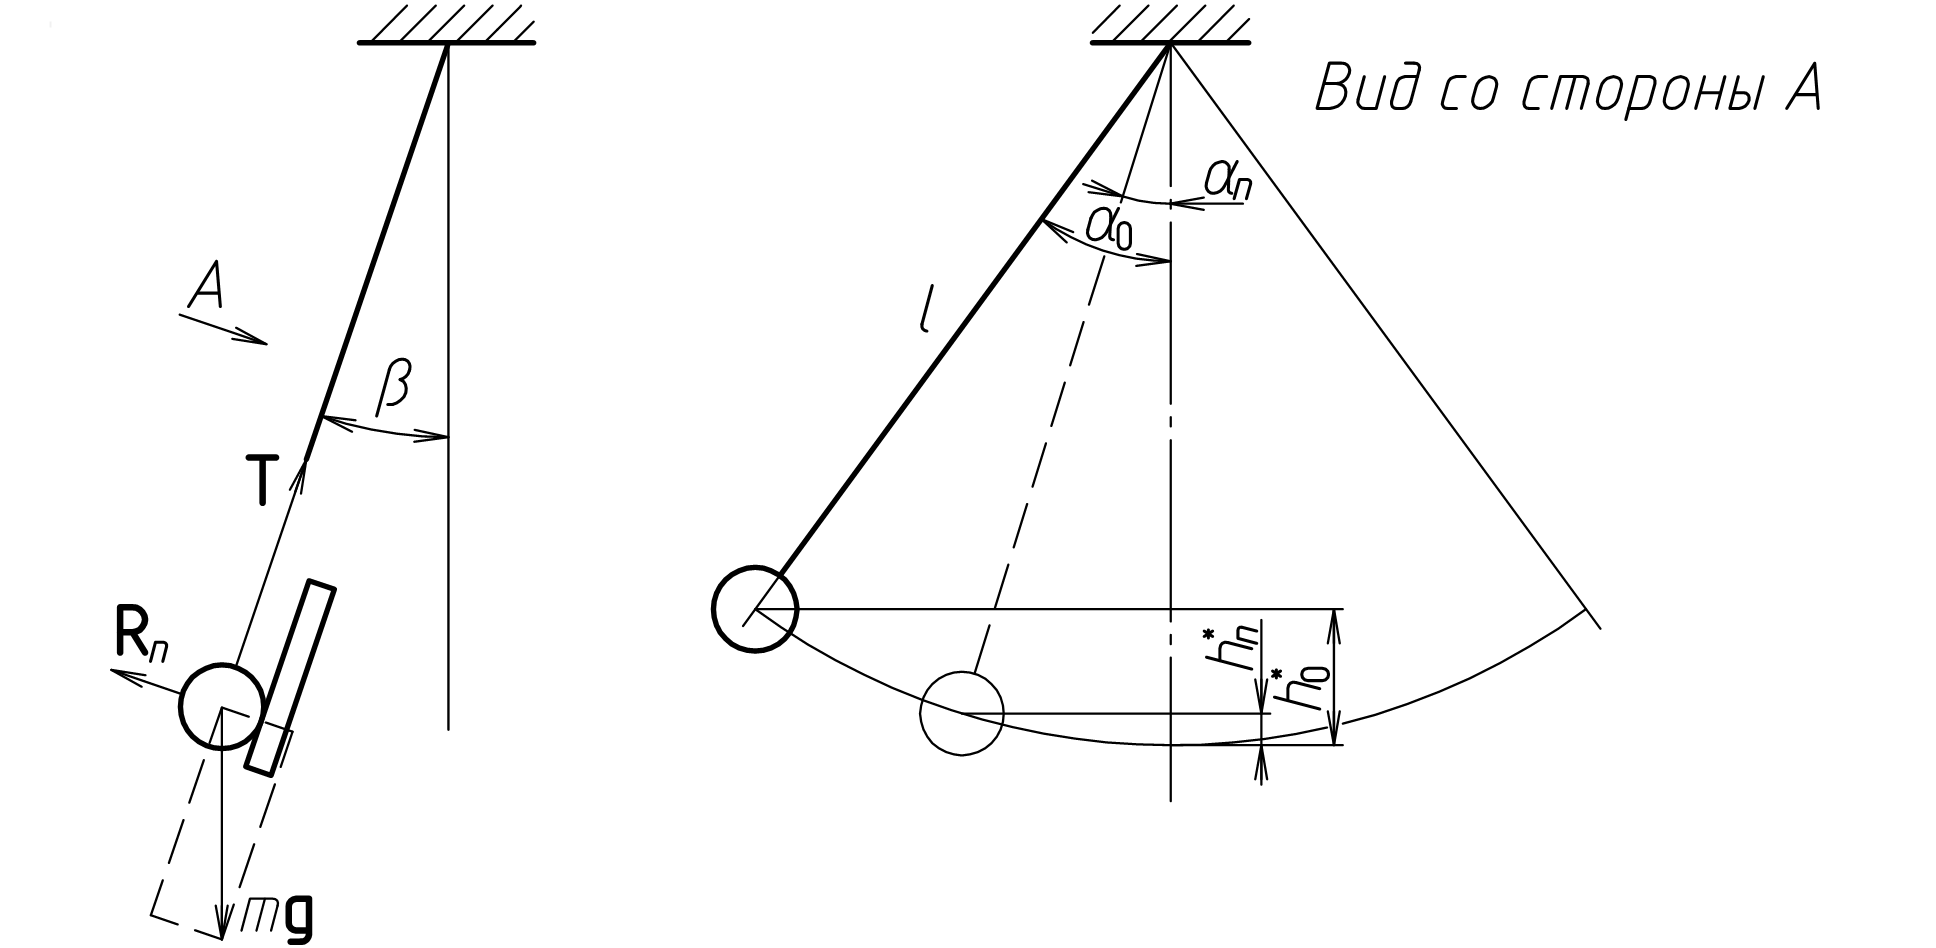
\includegraphics[scale = 0.26, keepaspectratio=true]{M8-RollingFrictionMachineForces}
\end{center}
\caption{Схема опыта \label{fig:m8-scheme}}
\end{figure}

В данной работе экспериментально определяется коэффициент трения качения пары <<шар "--- плоская пластина>>. полных колебаний измерить угол полного отклонения $\alpha_n$, то, в соответствии с законом изменения механической энергии, можно записать %я не понимаю смысла предложения, поэтому не знаю, нужна ли тут точка | Тут пропущена явно часть предложения.
% Исправь на "В данной работе экспериментально определяется коэффициент трения качения пары <<шар "--- плоская пластина>>. Если после N полных колебаний изменить угол...
\begin{equation}
\label{eq:m8-law-of-conservation}
mgh_0^\ast - mgh_n^\ast = A_\text{тр},
\end{equation}
где %некрасиво как-то, может ты можешь что-то придумать... хотя.... | Нормально
\begin{equation}
\label{eq:m8-h_0^ast}
h_0^\ast = 2l \sin^2 \frac{\alpha_0}{2} \cos \beta,
\end{equation}
\begin{equation}
\label{eq:m8-h_n^ast}
h_n^\ast = 2l \sin^2 \frac{\alpha_n}{2} \cos \beta.
\end{equation}
При малых углах (не превышающих $5 \degree$) $\sin x \approx x$ и %что-то approx не уменьшилось | Должно? А что не в порядке?
\begin{equation}
\label{eq:m8-h_0^ast-approx}
h_0^\ast = \frac{\alpha_0^2}{2} l \cos \beta,
\end{equation}
\begin{equation}
\label{eq:m8-h_n^ast-approx}
h_n^\ast = \frac{\alpha_n^2}{2} l \cos \beta.
\end{equation}

Работа сил трения рассчитывается как
\begin{equation}
\label{eq:m8-work-of-friction-force}
A_\text{тр} = M_\text{тр} \varphi,
\end{equation}
где $M_\text{тр}$ вычисляется в соответствии с выражением~\eqref{eq:m8-friction-moment}, а
\begin{equation}
\label{eq:m8-phi}
\varphi = 2 \pi l \frac{\alpha_0 + \alpha_n}{2} \cdot 4N \frac{1}{2 \pi r},
\end{equation}
где $r$ "--- радиус шара; \\ % Ты уверена, что в таких местах надо переносить? Хотя мы вроде решили, что да
$l$ "--- длина нити подвеса; \\
$\alpha_0$ "--- начальное отклонение шара от положения равновесия; \\
$\alpha_n$ "--- максимальное отклонение шара от положения равновесия после $N$ периодов.

Решая совместно уравнения (8.2)--(8.9) относительно $f_\text{к}$, получим расчетное соотношение %the same question as in m5
\begin{equation}
\label{eq:m8-f_k}
f_\text{к} = \frac{r}{\tg \beta} \cdot \frac{\alpha_0 + \alpha_n}{4N}.
\end{equation}


\subsection{Описание экспериментальной установки}
Общий вид экспериментальной установки приведен на рис.~\ref{fig:m8-equipment}. К основанию~\emph{1} прикреплена труба~\emph{2}, на которой смонтирован корпус~\emph{3} с червячной передачей, с помощью которой вращается кронштейн~\emph{4}. К кронштейну прикреплены шкалы~\emph{5} и~\emph{6} и штатив~\emph{7}, на который подвешен на нити шар~\emph{8}. На кронштейне же закреплена опорная пластина~\emph{9} и фотоэлектрический датчик~\emph{11}, управляющий миллисекундомером~\emph{12}. Червячная передача вращается с помощью ручки~\emph{10}.

\begin{figure}[h]
\begin{center}
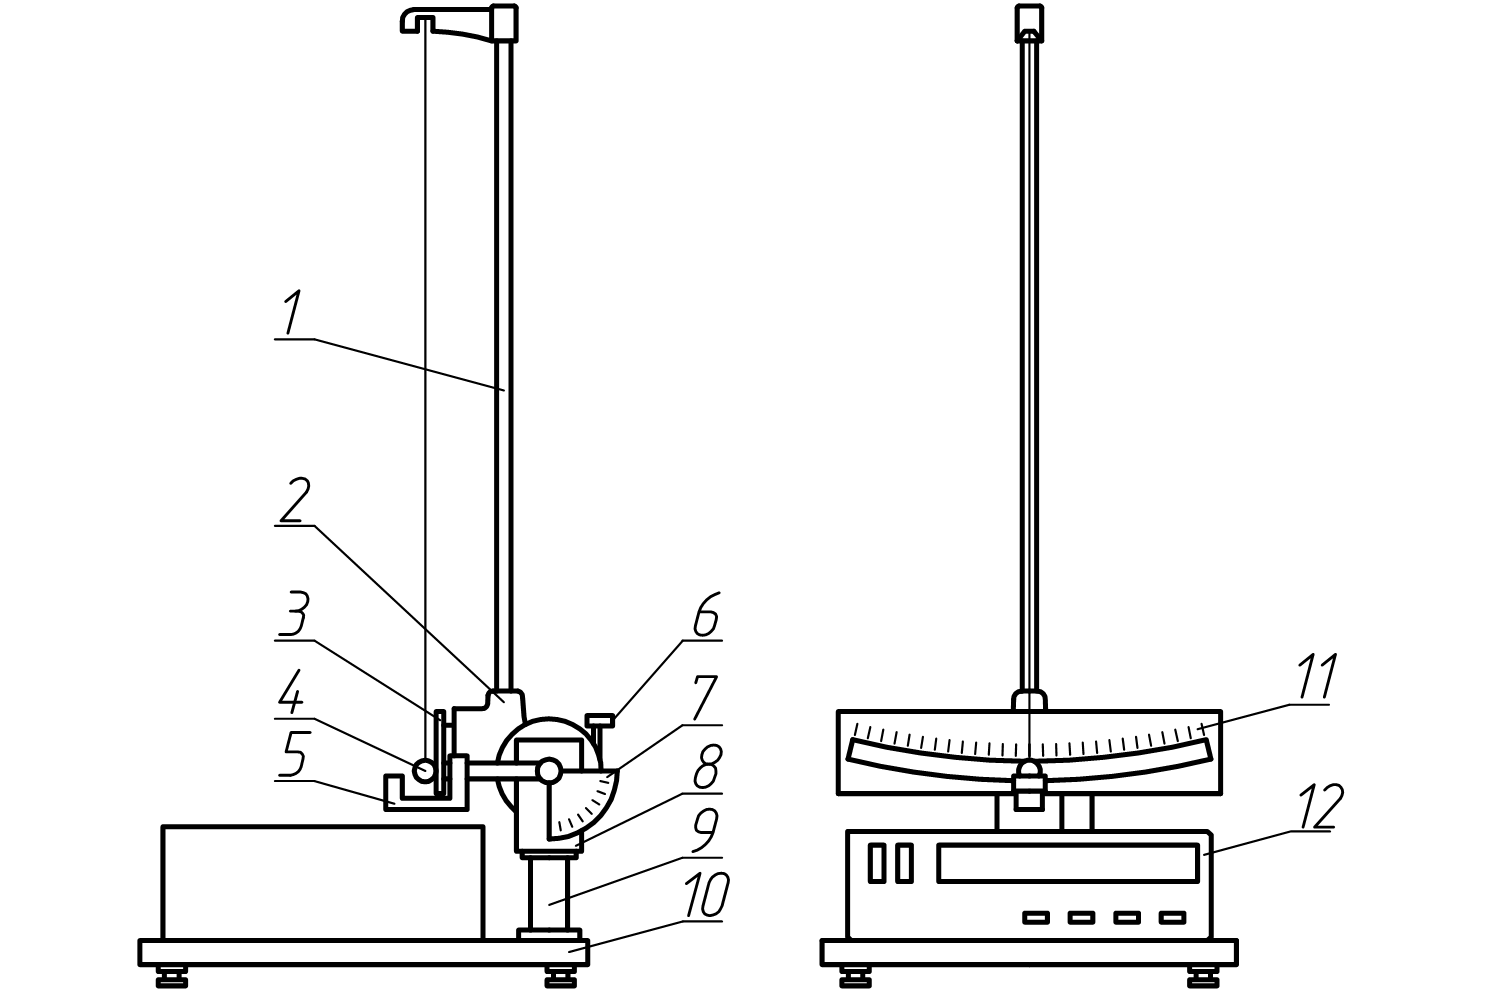
\includegraphics[scale = 0.35, keepaspectratio=true]{M8-RollingFrictionMachine}
\end{center}
\caption{Схема экспериментальной установки \label{fig:m8-equipment}}
\end{figure}


\subsection{Порядок выполнения работы}
\begin{enumerate}
\item Подготовьте таблицу~\ref{tab:m8-res-exp} в 4 экземплярах.

\begin{table}[h] %немного добавила линий в таблице, опираясь на порядок выполнения, хотя все равно неудобная она =(
\caption{\label{tab:m8-res-exp}}
\begin{center}
\begin{tabular}{|c|>{\centering\arraybackslash} m{0.7cm}|>{\centering\arraybackslash} m{0.7cm}|>{\centering\arraybackslash} m{0.7cm}|>{\centering\arraybackslash} m{0.7cm}|>{\centering\arraybackslash} m{0.7cm}|>{\centering\arraybackslash} m{0.7cm}|>{\centering\arraybackslash} m{0.7cm}|>{\centering\arraybackslash} m{0.7cm}|>{\centering\arraybackslash} m{0.7cm}|}
\hline
\multicolumn{10}{|c|}{$\beta = $} \\ \hline
$\alpha_0, \degree$ & \multicolumn{3}{c|}{} & \multicolumn{3}{c|}{} & \multicolumn{3}{c|}{} \\ \hline
$\alpha_n, \degree$ & & & & & & & & & \\ \hline
$t,~\Units{\text{c}}$ & & & & & & & & & \\ \hline
Число периодов $N$ & & & & & & & & & \\ \hline
\end{tabular}
\end{center}
\end{table}

\item Запишите в протокол измерений погрешности приборов.
\item Включите установку в сеть 220~\Units{В}.
\item Вращением ручки~\emph{10} отклоните штатив~\emph{7} на угол $\beta = 5\degree$ от вертикали.
\item Измерьте длину нити подвеса.
\item Нажмите кнопку <<Сброс>> секундомера.
\item Отклоните шар от положения равновесия на $\alpha_0 = 4\degree$ и отпустите. %ИЗМ: отпуститЕ | Я бы добавил "...его."
\item После совершения 10 полных колебаний измерьте визуально угол наибольшего отклонения по шкале и время по секундомеру, нажав после совершения нужного числа колебаний кнопку <<Стоп>> секундомера.
\item Измерения по пп.~6--8 повторите 3 раза.
\item Измерения по пп.~6--9 повторите для значений $\alpha_0$, равных $6\degree$ и $12\degree$.
\item Измерения по пп.~6--10 произведите для углов $\beta$, равных $10\degree$, $15\degree$, $20\degree$.
\item Результаты всех измерений запишите в таблицы.
\item С помощью выражения~\eqref{eq:m8-f_k} вычислите значения коэффициентов трения качения.
\item В соответствии с методикой, изложенной в разделе <<Введение>>, рассчитайте погрешности измерений коэффициента трения качения.
\item Постройте на одном графике зависимости $f_\text{к}(\alpha)$ при различных $\beta$.
\item Сформулируйте выводы.
\end{enumerate}


\subsection{Контрольные вопросы}
\begin{enumerate}
\item Что такое коэффициент трения качения? В чем его физический смысл? %ИЗМ: "качения, его физический" -> "качения? В чем его физический" | Ага
\item Сформулировать закон сохранения энергии. %сформулируйте? | Измени, правильно
\item Чем обусловлено возникновение трения качения?
\item Что такое систематическая и случайная погрешности измерения?
\end{enumerate}


\end{document}
